\documentclass[11pt]{article}
\usepackage{amsmath,amssymb,amsthm}
\usepackage{lipsum}
%Code found online which redefines amsmath matrices to include vertical bars (for e.g. augmented matrices)
\makeatletter
\renewcommand*\env@matrix[1][*\c@MaxMatrixCols c]{%
  \hskip -\arraycolsep
  \let\@ifnextchar\new@ifnextchar
  \array{#1}}
\makeatother
%end code
\newtheorem{thm}{Theorem}[section]
\newtheorem{defn}{Definition}[section]
\newcounter{enum}
\setcounter{enum}{0}
\newcommand{\m}[1]{\mathcal{#1}}
\newcommand{\lef}{\leftarrow}
\newcommand{\inner}[2]{\left\langle #1 \,\big |\, #2\right\rangle}
\title{CMIMC Power Round 2016}
\author{CMIMC Staff}
\usepackage{tikz}
\usetikzlibrary{automata,positioning}
\usepackage[top=2cm, left = 2cm, right = 2cm, bottom = 4cm]{geometry}
\usepackage{fancyhdr}
\pagestyle{fancy}
\lhead{}
\chead{\includegraphics[scale=0.12]{CMIMC-header.png}}
\rhead{}
\setlength{\headheight}{43pt}
\cfoot{Page \thepage}
\lfoot{}
\begin{document}\thispagestyle{empty}

\begin{center}

\vspace*{70pt}

\includegraphics[scale=0.23]{CMIMC-header.png}

\includegraphics[scale=0.35]{Power-Header.png}

\end{center}

\vspace{40pt}

\begin{center}
\includegraphics[scale=0.20]{instruction-header.png}
\noindent\rule{17.7cm}{2pt}
\end{center}

\vspace{10pt}

\begin{enumerate}
\item Do not look at the test before the proctor starts the round.

\item This test consists of several problems, some of which are short-answer and some of which require proofs.

\item Answers should be written and clearly labeled on sheets of blank paper. Each numbered problem should be \textit{on its own sheet}. If you have multiple pages, number them as well (e.g. 1/3, 2/3).

\item Write your team ID on the upper-right corner and the problem and page number of the problem whose solution you are writing on the upper-left corner on each page you submit. Papers missing these will not be graded. Problems with more than one submission will not be graded.

\item Write legibly. Illegible handwriting will not be graded.

\item In your solution for any given problem, you may assume the results of previous problems, even if you have not solved them. You may not do the same for later problems.

\item Problems are not ordered by difficulty. They are ordered by progression of content.

\item No computational aids other than pencil/pen are permitted.

\item If you believe that the test contains an error, submit your protest in writing to Porter 100.
\end{enumerate}

\newpage

\section{Introduction}

When working with computation on an abstract level, it is helpful to develop mathematical models for machines.  There are several mathematical models which work, but they all have similar characteristics:

\begin{itemize}

\item They must be simple to understand.

\item They must encompass many different computational tasks (though not necessarily all).

\item They must be hardware independent.  (Theoretical computer scientists don't really care about technical limitations; they instead care about which types of problems \textit{can} be solved by a computer.)

\end{itemize}

One such model of computation is known as a \textit{Deterministic Finite Automaton} (DFA).  DFAs are simplistic models of computation that still have deep theories and implications for computational theories in the real world.  In this power round, we will explore the underlying theory behind these mysterious models, solving interesting problems and proving fundamental results in automata theory along the way.

\section{Introduction to Languages}

Before we begin, we introduce the notation we shall be using to designate inputs to DFAs.  This section is mainly just definitions - manipulating languages will not come until later sections.

\begin{defn} An \emph{alphabet} is any finite, non-empty set of symbols. We often denote an alphabet by $\Sigma$.  Examples of alphabets are $\Sigma_1=\{0,1\}$ and $\Sigma_2=\{a,b,c\}$.\end{defn}

\begin{defn} A \emph{string} is any finite sequence of elements from an alphabet.  For any string $x$, $|x|$ denotes the number of characters in the string.  The empty string $\varepsilon$ represents the empty sequence.\end{defn}

\begin{defn}For an alphabet $\Sigma$, the notation $\Sigma^*$ denotes the set of all strings over $\Sigma$. For example, $\{0,1\}^*=\{\varepsilon,0,1,00,01,10,11,100,\dots\}$.\end{defn}

\begin{defn} A \emph{language} over an alphabet $\Sigma$ is any subset of $\Sigma^*$.\end{defn}

Now that we have some basic notation, it's time to move on to the meat of this power round.

\section{DFAs}

\begin{defn}A \emph{deterministic finite automaton} (DFA) is a mechanism that takes in a string as an input and either accepts or rejects it.  This is analogous to, say, a boolean function which takes in a string and outputs either \texttt{true} (i.e. accepts the string) or \texttt{false} (i.e. rejects it).\end{defn}

When drawn, DFAs look like a bunch of arrows and circles.  Here is an example of a DFA:

\begin{center}
\begin{tikzpicture}[node distance=2cm]
\node [state, initial] (q_0) {$q_0$};
\node [state] (q_1) [right of=q_0] {$q_1$};
\node [state, accepting] (q_2) [above right of=q_1] {$q_2$};
\node [state] (q_3) [below right of=q_1] {$q_3$};

\path [->]
(q_0) edge node [above] {0,1} (q_1)
(q_1) edge node [above left] {0} (q_2)
edge node [below left] {1} (q_3)
(q_2) edge [loop right] node {0,1} ()
(q_3) edge [loop right] node {0,1} ();
\end{tikzpicture}
\end{center}

Each circle represents a \emph{state}. A state with two circles is an \emph{accepting state}, which means the DFA will accept if the string ends up there. Formally, a DFA over an alphabet $\Sigma$ is defined as a finite set of states (with one start state and some of which can be accepting states), each with an arrow pointing to another state for each element of $\Sigma$. For a DFA, the language that it \emph{admits} is the language of all strings over $\Sigma$ that accept when inputted into the DFA.

To read a DFA, start with the string in the state indicated by the ``start" arrow. Look at the first letter in the string, then follow the arrow corresponding to that letter to the next state. From that state, follow the arrow corresponding to the second letter of the string, and so on until the string has no more letters. At that point, the DFA accepts if you are in an accepting state and rejects otherwise.

For example, let's input the string $1011$ into the above DFA. It starts at $q_0$. The first letter is $1$, so move to $q_1$. The second letter is $0$ so move to $q_2$. The third letter is $1$ so move to $q_2$. The fourth letter is $1$, so move to $q_2$. There are no more letters left, and we are in an accepting state, so this DFA will accept the string $1011$.

\begin{enumerate}
\item {[}\textbf{2}{]} Consider the following DFA:

\begin{center}
\begin{tikzpicture}[node distance=2cm]
\node [state, initial] (q_0) {$q_0$};
\node [state] (q_1) [right of=q_0] {$q_1$};
\node [state, accepting] (q_2) [right of=q_1] {$q_2$};
\node [state] (q_3) [right of=q_2] {$q_3$};

\path [->]
(q_0) edge node [above] {1} (q_1)
      edge [loop above] node {0} ()
(q_1) edge node [above] {0} (q_2)
      edge [loop above] node {1} ()
(q_2) edge node [above] {0,1} (q_3)
(q_3) edge [loop right] node {0,1} ();
\end{tikzpicture}
\end{center}

For each of the following strings, indicate whether the DFA accepts or rejects:

\begin{center}
\begin{tabular}{c|c|c}
string & accepts & rejects \\
\hline
0000 &  & \\
\hline
1111 &  & \\
\hline
0010 &  & \\
\hline
0110 &  & \\
\hline
0100 &  & \\
\end{tabular}
\end{center}

\item Consider the following DFAs.  In simplest terms, what languages would they accept?

\begin{enumerate}

\item {[}\textbf{2}{]} See below.

\begin{center}
\resizebox{200pt}{!}{
\begin{tikzpicture}[shorten >=1pt,node distance=2cm,on grid,auto] 
   \node[state,initial] (q_0)   {$q_0$}; 
   \node[state] (q_1) [above right=of q_0] {$q_1$}; 
   \node[state] (q_2) [below right=of q_0] {$q_2$}; 
   \node[state,accepting](q_3) [below right=of q_1] {$q_3$};
    \path[->] 
    (q_0) edge  node {0} (q_1)
          edge  node [swap] {1} (q_2)
    (q_1) edge  node  {1} (q_3)
          edge [loop above] node {0} ()
    (q_2) edge  node [swap] {0} (q_3) 
          edge [loop below] node {1} ()
		(q_3) edge [loop right] node {0,1} ();
\end{tikzpicture}
}
\end{center}

\item {[}\textbf{4}{]} See below.

\begin{center}
\resizebox{300pt}{!}{
\begin{tikzpicture}[shorten >=1pt,node distance=2cm,on grid,auto] 
   \node[state,initial] (q_0)   {$q_0$}; 
   \node[state] (q_1) [above right=of q_0] {$q_1$}; 
   \node[state] (q_2) [below right=of q_0] {$q_2$}; 
   \node[state] (q_3) [right=of q_1] {$q_3$};
	 \node[state] (q_4) [right=of q_2] {$q_4$};
	 \node[state,accepting] (q_5) [below right=of q_3] {$q_5$};
    \path[->]
    (q_0) edge  node {0} (q_1)
          edge  node [swap] {1} (q_2)
    (q_1) edge  node {0} (q_3)
          edge [bend left = 6] node {1} (q_2)
    (q_2) edge [bend left = 6] node {0} (q_1) 
          edge  node  {1} (q_4)
		(q_3) edge  node  {0} (q_5)
		      edge  node [above right = 0.25cm and 0.35cm] {1} (q_2)
	  (q_4) edge  node [below right = 0.25cm and 0.35cm] {0} (q_1)
		      edge  node  {1} (q_5)
	  (q_5) edge [loop right] node {0,1} ();
\end{tikzpicture}
}
\end{center}

\end{enumerate}

\item For each of the problems below, construct a DFA which accepts the given language.  You do not need to prove that your submission works.

\begin{enumerate}

\item {[}\textbf{2}{]} $L_1 = \{w\in\{0,1\}^*\,|\,w=001\}$

\item {[}\textbf{2}{]} $L_2 = \{w\in\{a,b\}^*\,|\,w\text{ has even length}\}$

\item {[}\textbf{6}{]} $L_3=\{w\in\{0,1\}^*\setminus\varepsilon\,|\,w\text{ when interpreted as an integer in binary is divisible by 5}\}$

\end{enumerate}

\item {[}\textbf{5}{]} Let $D$ be a DFA with exactly three states.  Suppose this DFA accepts the string $000$ but \textit{not} the empty string $\varepsilon$.  What is the smallest positive integer $k>3$ such that $D$ \textit{must} also accept $0^k$? (Here, exponentiation is shorthand for repetition; for example, $0^4$ represents the string $0000$.) Prove that your $k$ is minimal.

\end{enumerate}

\section{Languages and Regularity}

\par It is useful to understand both the capabilities and limitations of any model of computation such as a DFA.  This roughly translates to determining which problems either do not have solutions or have solutions which extend beyond the scope of the aforementioned model of computation.  This next section, as well as the ones which succeed it, help develop the theory behind what these DFA machines can actually do.

\begin{defn}We say that a language $\Sigma^*$ is \textit{regular} if there exists a DFA $D$ which accepts all words $w\in\Sigma^*$ and rejects all words $w_0\not\in\Sigma^*$.  If this is the case, we say that $D$ \textit{decides} the language or is a \textit{decider} for the language.  (Either phrase is fine.)
\end{defn}

As an example, the language \[L=\{x\in\{0,1\}^*\,\,\mid\,\,\text{the second digit from the left is a 0}\}\] is regular, because the DFA pictured in the previous section is a decider for $L$.

\begin{enumerate}
\setcounter{enumi}{\theenum}

\item {[}\textbf{3}{]} Is any language consisting of a finite number of words (sometimes called a ``finite language'') regular?

\setcounter{enum}{\theenumi}
\end{enumerate}

\par Determining whether a language is regular is somewhat straightforward: construct a DFA which decides it!  This technique is the basis for almost all problems which ask you to show that some language is regular.  Proving a language is irregular, however, is a bit more difficult; one has to come up with a precise argument that works against \textit{all} possible DFAs.  The key to doing this relies in the `F' in DFA.  The following problem highlights the general technique.

\begin{enumerate}
\setcounter{enumi}{\theenum}

\item Consider the language $L=\{0^n1^n:n\in\mathbb{N}\}$.

\begin{enumerate}

\item {[}\textbf{2}{]} Suppose $D$ is a DFA with $n$ states which decides $L$.  Furthermore, let $S$ be a set of consisting of $k$ words $w\in \{0,1\}^*$.  What is the smallest value of $k$ such that for all such sets $S$, there exist two words in $S$ which land in the same state at the end of the simulation?  Provide brief justification.

\item {[}\textbf{4}{]} Using this, show that $L$ is irregular, i.e. show that $D$ does not exist.

\end{enumerate}

\setcounter{enum}{\theenumi}
\end{enumerate}

\par Before we move on to the main meat of the section regarding regularity (the problems), an interlude.  Up until now, we have been informal about what exactly a DFA is in a mathematical sense.  We have refrained from doing this in order to prevent definitions from interfering with intution.  However, some of the problems from this point forward benefit greatly from formal notation, so we will introduce it here.


\begin{defn}
Formally, a deterministic finite automaton $M$ is a $5$-tuple \[M=(Q,\Sigma,\delta, q_0, F),\] where

\begin{itemize}

\item $Q$ is the (finite) set of states of $M$;

\item $\Sigma$ is the alphabet of the strings inputted to and processed by $M$;

\item $\delta:Q\times\Sigma\mapsto Q$ is a transition function which details exactly how the states and alphabet function with each other (in other words which arrows point to which states);

\item $q_0\in Q$ is the start state of $M$;

\item $F\subseteq Q$ is the set of accepting states of $M$.

\end{itemize}

\end{defn}

\par While formal notation is not necessary for completing the rest of this Power Round, it may help make some of the solutions easier to write.

\begin{enumerate}
\setcounter{enumi}{\theenum}

\item {[}\textbf{4}{]} Show that the language $\{1^{2^n}\,|\,n\in\mathbb{N}\}$ is irregular.

\item The above two problems demonstrate the usefulness of elementary combinatorics to prove results regarding regularity.  Using these basic ideas, we can construct very powerful results in automata theory.  One of the most fundamental is stated below.

\begin{thm}[Pumping Lemma] Let $L$ be a regular language.  Then there exists an integer $P\geq 1$ such that any $w\in L$ with $|w|\geq P$ can be written as $w=xyz$ with $y$ not equal to the empty string such that

\begin{itemize}

\item $|xy|\leq P$, and

\item for all integers $i\geq 0$, the string $xy^iz$ is also in $L$.

\end{itemize}
\end{thm}

In this problem we give a proof of the lemma and then see how it can be used to solve some regularity problems.

\begin{enumerate}

\item {[}\textbf{2}{]} Suppose $M$ is a DFA which decides $L$.  Let $p$ be the number of states of $M$.  Consider an input \[s=s_1s_2\ldots s_n\qquad\text{with}\quad n\geq p.\] Let $q_k$ be the state the automata is in after reading the character $s_k$.  Show that there exist integers $0\leq i < j\leq p$ such that $q_i=q_j$.

\item {[}\textbf{6}{]} Let $i$ and $j$ be as above.  Define \[x=s_1s_2\ldots s_i,\quad y=s_{i+1}\ldots s_j,\quad\text{and}\quad z = s_{j+1}\ldots s_n.\] Show that these $x$, $y$, and $z$ fit the description given in the Pumping Lemma, where $P=p$.

\item {[}\textbf{4}{]} Using the Pumping Lemma, show that the language \[L=\{s\,|\,|s|\text{ is a prime number}\}\] is not regular.

\end{enumerate}

\item One natural question to ask is how regularity behaves under certain string and set operations.  These might include the union and intersection of two languages as well as their concatenation.  It turns out that regular languages are closed under many different kinds of operations.  The following problems will ask to prove closure of regularity under different types of operations.

\begin{enumerate}

\item \textbf{COMPLEMENT} {[}\textbf{2}{]}: Let $L$ be a regular language over the alphabet $\Sigma$, and set \[L^c = \{x\in\Sigma^*\,|\, x\not\in L\}.\] Prove that $L^c$ is also regular.

\item \textbf{INTERSECTION} {[}\textbf{6}{]}: Suppose $A$ and $B$ are two regular languages over a common alphabet $\Sigma$.  Prove that \[A\cap B = \{x\in\Sigma^*\,|\,x\in A\text{ and }x\in B\}\] is also regular.

\item \textbf{UNION} {[}\textbf{6}{]}: Suppose $A$ and $B$ are two regular languages over a common alphabet $\Sigma$.  Prove that \[A\cup B = \{x\in\Sigma^*\,|\,x\in A\text{ or }x\in B\}\] is also regular.

\item\textbf{SET DIFFERENCE} {[}\textbf{2}{]}: Suppose $A$ and $B$ are two regular languages over a common alphabet $\Sigma$.  Prove that \[A\setminus B = \{x\in\Sigma^*\,|\,x\in A\text{ and }x\not\in B\}\] is also regular.

\end{enumerate}

There are other set operations (e.g. concatenation) that can also be shown to be closed under regularity, but doing so requires the notion of a non-deterministic finite automaton, which is beyond the scope of this power round.

\item {[}\textbf{8}{]} For any language $L\in\{0,1\}^*$, define a language $L_0$ which consists of the set of words of the form \[a_1s_{1,2}a_2s_{2,3}a_3\ldots a_{k-1}s_{k-1,k}a_k\] where $a_1a_2a_3\ldots a_k$ is a word in $L$ and $s_{i,j}$ is $1$ when $a_i\neq a_j$ and zero otherwise. For example, the word $1101$ in $L$ corresponds to the word $1011011$ in $L_0$.

\par Suppose $L$ is regular.  Must $L_0$ also be regular?
\setcounter{enum}{\theenumi}
\end{enumerate}

\section{DFA Minimization}

\par One of the biggest overall themes in the field of computer science is optimization.  If wew have a program that can solve a problem but does so in exponential time (e.g. the number of steps needed to solve the problem on input of length $n$ is roughly $2^n$), then the algorithm isn't really that practical!  Computer scientists aim to design and implement processes which are efficient in some sense.  As a result, it might be beneficial to see how we can explore this type of minimization in DFAs.  The most natural way to do so involves looking at the number of states for a DFA which decides some language $L$. 

\begin{enumerate}
\setcounter{enumi}{\theenum}

\item {[}\textbf{2}{]} Below is a picture of a DFA which accepts some language $L$.  Although this DFA is a decider for $L$, it is somewhat inefficient.  Propose two modifications to this DFA so that it still decides $L$ but requires fewer states to do so.

\begin{center}
\begin{tikzpicture}[node distance=1.5cm]
\node [state, initial] (q_0) {$q_0$};
\node [state] (q_1) [right = of q_0] {$q_1$};
\node [state] (q_2) [right = of q_1] {$q_2$};
\node [state, accepting] (q_3) [right = of q_2] {$q_3$};
\node [state] (q_4) [below = of q_3] {$q_4$};
\node [state, accepting] (q_5) [left  = of q_4] {$q_5$};
\path [->]
(q_0) edge node [above] {0,1} (q_1)
(q_1) edge node [above] {0,1} (q_2)
(q_2) edge node [above] {0,1} (q_3)
(q_3) edge node [right] {0,1} (q_4)
(q_4) edge node [below] {0,1} (q_5)
(q_5) edge node [left]  {0,1} (q_2);
\end{tikzpicture}
\end{center}

\item {[}\textbf{8}{]} Consider the language \[L=\{0^n1^m\,|\,n-m\equiv 0\pmod 3\}.\] Note that this language is a more general version of one that we've explored before.  However, in fact this language is regular!  What is the smallest number of states needed in a DFA that decides $L$? (Your answer must both establish a minimum number of states and show that this minimum is achievable.)

\item

\begin{enumerate}

\item {[}\textbf{4}{]} Define \[\mathcal{L}_n=\{x\,\mid\, x\in\{0,1\}^*\text{ and the }n^{\text{th}}\text{-symbol from the left is a 1 }\}.\]  Show that there is some constant number $c$ (independent of $n$) such that there is a DFA that accepts $\mathcal{L}_n$ with at most $n+c$ states.

\item {[}\textbf{5}{]} Define \[\mathcal{R}_n=\{x\,\mid\, x\in\{0,1\}^*\text{ and the }n^{\text{th}}\text{-symbol from the right is a 1 }\}.\]  Show that any DFA that accepts $\mathcal{R}_n$ has at least $2^n$ states.

\end{enumerate}

\setcounter{enum}{\theenumi}
\end{enumerate}

\par It turns out that DFAs are simple enough in nature that we can algorithmically construct a minimal DFA for any given language $L$!  (The only caveat is that we need to find some DFA which decides $L$ first before applying this algorithm, but that's a worthy trade-off.)  To explore this idea, we need to develop the notion of equivalence classes.

\begin{defn}
Let $\Sigma$ be an alphabet, and let $A$ be any language over $\Sigma^*$.  For any word $v\in \Sigma^*$, let \[S_v(A)=\{w\in\Sigma^*\,\mid\, vw\in L\} .\] We then say that two strings $x,y\in\Sigma^*$ are \textit{equivalent} iff $S_x(A) = S_y(A)$.  We denote this mathematically through the relation $x\equiv_A y$.  Note that $\equiv_A$ is an equivalence relation, and so we may refer to the equivalence classes\footnote{For any set $X$ equipped with an equivalence relation $\sim$ and for any $a$ in $X$, we say that the equivalence class of $a$ is the subset of all elements $x\in X$ for which $x\sim a$.  It follows that these equivalence classes partition $X$ into subsets; we then define the number of equivalence classes of $\sim$ as the number of subsets in this partition.} of $A$.
\end{defn}

\par There exists a similar notion of equivalence with regards to DFAs.

\begin{defn}
Given a DFA $M=(Q,\Sigma,\delta, q_0, F)$, we say that two strings $x,y\in\Sigma^*$ are \textit{indistinguishable} iff $\delta*(q_0,x)=\delta^*(q_0,y)$.  In other words, the state reached by $M$ on input $x$ is the same as the state reached by $M$ on input $y$.  We denote the notion of equivalence as $x\equiv_M y$.  Just as above, note that $\equiv_M$ is an equivalence relation and so we may refer to the equivalence classes of $M$.
\end{defn}

\begin{enumerate}
\setcounter{enumi}{\theenum}

\item {[}\textbf{2}{]} Let $L=\{0^n1^n\,|\, n\in\mathbb{N}\}$.  What is $S_{111100}(L)$?

\item {[}\textbf{3}{]} Suppose $M$ is a DFA with $N$ states.  At most how many equivalence classes can $M$ have?  What is an example of a DFA $M$ for which equality does not hold?

\item {[}\textbf{5}{]} Show that the notions of equivalency and indistinguishability are identical.  In other words, let $M$ be a DFA and let $A=L(M)$.  Then for any $x,y\in\Sigma^*$, if $x\equiv_M y$, then $x\equiv_A y$.

\setcounter{enum}{\theenumi}
\end{enumerate}

We now have enough background knowledge to state an important result.

\begin{thm}[Myhill-Nerode]A language $A$ is regular iff the equivalence relation $\equiv_A$ has a finite number of equivalence classes.  Furthermore, there exists some DFA $M$ with $L(M)=A$ such that every state of $M$ uniquely corresponds to an equivalence class of $\equiv_A$.
\end{thm}

\begin{enumerate}
\setcounter{enumi}{\theenum}

\item {[}\textbf{8}{]} Prove this theorem.

\setcounter{enum}{\theenumi}
\end{enumerate}

Using this theorem, we now can construct an algorithm for minimizing any DFA!  The algorithm is as follows.  (Note: in this algorithm, we use the official definition of a DFA given in the previous section.)

\begin{itemize}

\item Draw a table for all pairs of states $(Q_i,Q_j)$ (not just those which are connected directly).  Initially, these pairs will be unmarked.

\item Mark all state pairs $(Q_i,Q_j)$ with the property that $Q_i\in F$ and $Q_j\not\in F$ and mark them.

\item For some input $A$, if there exist states $Q_i$ and $Q_j$ with the property that $(\delta(Q_i,A),\delta(Q_j,A))$ is marked, then mark the pair $(Q_i,Q_j)$.  Repeat this until there are no more states that can be marked.

\item Combine all the unmarked pairs of states in the reduced DFA.  Return this new DFA.  (For example, if $\{a,b\}$, $\{b,c\}$, and $\{c,a\}$ are all unmarked, combine the states $a,b,c$ into one big state.)

\end{itemize}

\newpage

\begin{enumerate}
\setcounter{enumi}{\theenum}

\item {[}\textbf{4}{]} Perform this algorithm on the following DFA.  What is the result?

\begin{center}
\begin{tikzpicture}[node distance = 2 cm]
\node [state, initial] (q_0) {$q_0$};
\node [state] (q_1) [above = of q_0] {$q_1$};
\node [state, accepting] (q_2) [right = of q_0] {$q_2$};
\node [state, accepting] (q_3) [right = of q_1] {$q_3$};
\node [state, accepting] (q_4) [right = of q_2] {$q_4$};
\node [state] (q_5) [right = of q_3] {$q_5$};
\path[->]
(q_0) edge [bend left = 6] node [left] {0} (q_1)
      edge node [below] {1} (q_2)
(q_1) edge [bend left = 6] node [right] {0} (q_0)
      edge node [above] {1} (q_3)
(q_2) edge node [below] {0} (q_4)
      edge node [above left = -0.60cm and 0.4cm] {1} (q_5)
(q_3) edge node [above right = 0.70cm and -0.8cm] {0} (q_4)
      edge node [above] {1} (q_5)
(q_4) edge [loop right] node {0} (q_4)
      edge node [left] {1} (q_5)
(q_5) edge [loop right] node {0,1} (q_5);
\end{tikzpicture}
\end{center}

\item {[}\textbf{6}{]} Show using the Myhill-Nerode Theorem that this procedure produces a DFA with the minimal number of states.

\end{enumerate}

\end{document}

\newpage

\begin{center}
\begin{tikzpicture}[node distance=2cm]
\node [state, initial] (q) {$q$};
\node [state, accepting] (q_0) [below left of=q] {$q_0$};
\node [state] (q_1) [below right of=q] {$q_1$};
\node [state] (q_2) [below right of=q_0] {$q_2$};
\node [state] (q_4) [below left of=q_2] {$q_4$};
\node [state] (q_3) [below right of=q_2] {$q_3$};

\path [->]
(q)   edge node [above left] {0} (q_0)
      edge node [above right] {1} (q_1)
(q_0) edge [loop left] node {0} (q_0)
      edge node [above] {1} (q_1)
(q_1) edge node [above left] {0} (q_2) 
      edge [bend right = 6] node [left = 0.01cm] {1} (q_3) % bend slightly left
(q_2) edge node [above right] {1} (q_0)
      edge node [above left] {0} (q_4)
(q_3) edge [bend right = 6] node [right = 0.01cm] {0} (q_1) % bend slightly right
      edge node [above right] {1} (q_2)
(q_4) edge [loop left] node {1} (q_4)
      edge node [below] {0} (q_3);
\end{tikzpicture}
\end{center}
